\documentclass{article}
\usepackage{blindtext}
\usepackage[a4paper, total={6.5in, 10in}]{geometry}

\usepackage{amsmath}
\usepackage{mathtools}
\usepackage{caption}
\usepackage{subcaption}
\usepackage{mathrsfs}

\usepackage{dcolumn}% Align table columns on decimal point
\usepackage{bm}% bold math
\usepackage{float}
\usepackage{braket}
\usepackage{xcolor}
%\usepackage{caption}
%\usepackage{subcaption}
\usepackage{graphicx}% Include figure files
\usepackage{dcolumn}% Align table columns on decimal point
\usepackage{bm}% bold math


\newcommand{\Comment}[1]{\textcolor{red}{[#1]}}
\bibliographystyle{apalike}

\begin{document}
\title{Supplemental Material:}% Force line breaks with \\

\author{Bipul Pandey, Peter B. Littlewood}

\date{\today}% It is always \today, today,
             %  but any date may be explicitly specified
\maketitle

\section{Electron and Boson Green's Function}
In our single electron two site Holstein problem, we look at the electron addition spectra. For this problem, the ground state is the fock vacuum $|0\rangle$ which doesn't have any fermion or boson in it. We will now define the electron and boson Green's function for this problem with $|0\rangle$ as the ground state.

\textbf{The electron Green's function: } In retarded-time formalism \cite{kas_cumulant_2014} for a two orbitals ($n =\pm$) system described by \eqref{Holstein}, with $\{,\}$ as the anti-commutator, $c_n^\dagger /c_n$ as the electron creation/annihilation operators, and ${|0\rangle}$ as the fock vacuum, the RT one-particle electron addition Green's function $G(n;t)$ is the probability amplitude for a particle injected into orbital 'n' to be in 'n' after time t \cite{goodvin_greens_2006}.
\begin{equation}
\begin{aligned}
    G(n;t) &= -i \theta(t)\left\langle 0|\{c_n(t) ,{c_n^{\dagger}}\}|0\right\rangle\\
    &= -i \theta(t)\left\langle 0|\{e^{iHt}c_n e^{-iHt} ,{c_n^{\dagger}}\}|0\right\rangle
\end{aligned}
\label{Greens def}
\end{equation}
 The non-interacting($g=0$) or bare electron Green's function $G_o(\pm,t)$, given the bare energy eigenvalues $\varepsilon_{\pm}$ of  $H_o$ and evolution time 't', is as follows;
\begin{equation}
\begin{aligned}
    G_o(\pm,t) &=-i \theta(t)\left\langle 0|\{e^{iH_ot}c_n e^{-iH_ot} ,{c_n^{\dagger}}\}|0\right\rangle\\
    &=-i\theta(t) e^{-i\varepsilon_\pm t} 
\end{aligned}
    \label{Bare electron greens}
\end{equation} 

\textbf{The Boson Green's function: }
In RT formalism, with $[ , ]$ as the commutator, $b_N^\dagger/b_N$ as the boson creation/annihilation operators, ${|0\rangle}$ as the fock vacuum, the RT one-particle boson addition Green's function $D(N=\pm;t)$ is the probability amplitude for a 'N' type boson to remain in 'N' type after time t
\begin{equation}
\begin{aligned}
    \mathcal{D}(N,t) &= -i \theta(t)\langle 0|[b_N(t) ,{b_N^{\dagger}}]|0\rangle\\
     &= -i \theta(t)\langle 0|[e^{iHt}b_N e^{-iHt} ,{b_N^{\dagger}}]|0\rangle
\end{aligned}
\label{Boson greens}
\end{equation}
The non-interacting($g=0$) or bare boson operator for dispersionless bosons of frequency $\omega_o$ is given by;
\begin{equation}
\begin{aligned}
    \mathcal{D}(\pm,t) &=-i \theta(t)\langle 0|[e^{iH_\pm t}b_N e^{-iH_\pm t} ,{b_N^{\dagger}}]|0\rangle\\
    &=-i \theta(t)e^{- i\omega_o t}
\end{aligned}
    \label{Bare boson greens}
\end{equation} 


\section{Spectral Function and Improper convergence of Delta Function}
In our work, the photo-emission spectral function $A(m,n;\omega)$ evaluated on the frequency axis is defined as;
 \begin{equation*}
     A(m,n;\omega) = \frac{1}{\pi} |\text{Im}G(m,n;\omega)|
 \end{equation*}
 This absolute valued definition of spectral function differs from the traditional definition and is necessary in numerical application because of the finiteness of the time axis. We explain this further in this section. The retarded time bare electron Green's function in frequency space is defined as;
\begin{equation}
\begin{aligned}
    G_o(k,\omega) &= \lim_{\eta\rightarrow0^+}\frac{1}{\omega -\varepsilon_k +i\eta}\\
    & =\mathscr{P}\Big[\frac{1}{\omega-\varepsilon_k} \Big] - i\pi\delta(\omega-\varepsilon_k)
\end{aligned}
\end{equation}
Here, $\mathscr{P}$ represents the principal value of the function it is acting on. We see that the imaginary part of this $G_o(k,\omega)$ has the poles at the energy eigenvalues $\varepsilon_k$ of the non-interacting part of Hamiltonian. From this, the traditional definition of the spectral function emerges;
\begin{equation}
    A_o(k,\omega) = -\frac{1}{\pi} \text{Im}(G_o(k,\omega)
    \label{traditional}
\end{equation}
Assuming a smooth transition from non-interacting to interacting system, we can extend this expression's validity to define interacting system's spectral function;
\begin{equation}
    A(k,\omega) = -\frac{1}{\pi} \text{Im}(G(k,\omega)
\end{equation}

In the context of Dirac Delta function we often use the following relationship:
\begin{equation}
\begin{aligned}
    \lim_{\eta\rightarrow 0^+} \frac{1}{x\pm i \eta} &=\lim_{\eta\rightarrow 0^+} \frac{x}{x^2+ \eta^2} \quad\mp\quad\lim_{\eta\rightarrow 0^+}  i\pi \frac{\eta}{\pi(x^2 + \eta^2)}\\
    & =\qquad \,\,\mathscr{P}\Big[\frac{1}{x} \Big] \qquad\mp\qquad i\pi\delta(x)
\end{aligned}
\end{equation}

The delta function in the imaginary part originates from the limit-definition (Sokhotski-Plemelj Theorem or Kramers Kronig Relations) of the function in the line right above it and hence is an idealization when it comes to numerical implementation. This is because in numerical implementation, explicitly demanding that $\eta$ must go to zero only from the positive side of the number line (since we demand $\eta\rightarrow0^+$) for a continuous function (bare electron green's function) is notoriously difficult. On top of this, the negative side then requires a sign flip in the definition of the delta function. Now, we no longer have a unified definition of delta function but rather a piece wise definition. This is still manageable when we have a single delta function i.e bare electron Green's function in any one half of the real line. But when we use the bare electron Green's function to compute actual Green's function in symmetric time domain and convert back to frequency domain, we now notice that we need to enforce this piece-wise definition of Green's function at every given frequency point. Furthermore, since there is a cutoff ($t_{max}$) in time, this manifests as oscillations in the frequency space in the order of $t^{-1}_{max}$. We are now at an impasse. We need a large $t_{max}$ (ideally $t_{max}\rightarrow \infty$) to properly capture the Green's function decay. But $t_{max}$ needs to be some large finite value for numerical implementation which manifests as violent small energy oscillation. In order to bypass this and reproduce correct answer for non-interacting as well as interacting fermionic systems, we can redefine the limit-definition of the function with an absolute value as follows;
\begin{equation}
\begin{aligned}
    \lim_{\eta\rightarrow 0} \frac{1}{x\pm i \eta} &=\lim_{\eta\rightarrow 0} \frac{x}{x^2+ \eta^2} \quad\mp\quad\lim_{\eta\rightarrow 0}  i\pi\Big| \frac{\eta}{\pi(x^2 + \eta^2)}\Big|\\
    & =\qquad \,\,\mathscr{P}\Big[\frac{1}{x} \Big] \qquad\mp\qquad i\pi\delta(x)
\end{aligned}
\end{equation}

Doing so, we now get a consistent single definition of the delta function on both sides of the number line. This manifests in our definition of the spectral function.

\begin{equation}
    A(k,\omega) = \frac{1}{\pi}|G(k,\omega)|
    \label{absolute}
\end{equation}

\begin{figure}
\centering
\begin{subfigure}{.5\textwidth}
  \centering
  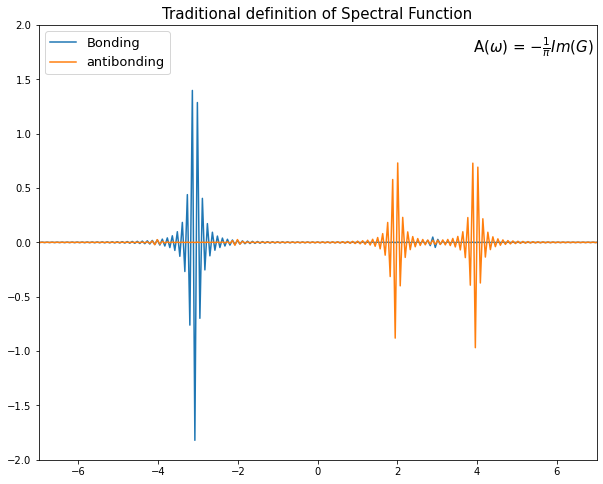
\includegraphics[width=.9\linewidth]{Traditional_defn.png}
  \caption{Traditional definition from equation \eqref{traditional}}
  \label{fig:sub1}
\end{subfigure}%
\begin{subfigure}{.5\textwidth}
  \centering
  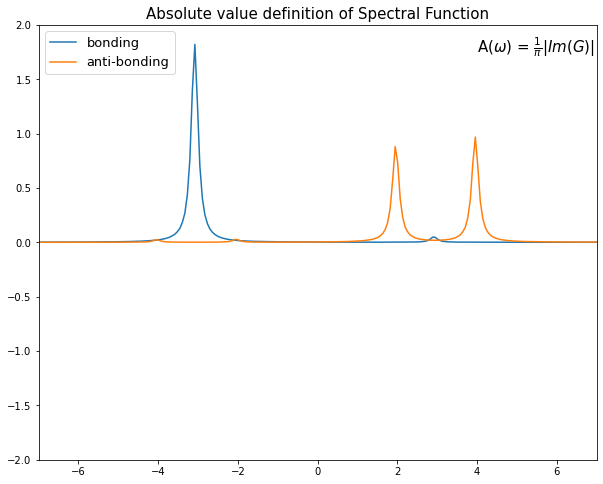
\includegraphics[width=.9\linewidth]{Absolute_defn.png}
  \caption{Absolute value definition from equation \eqref{absolute}}
  \label{fig:sub2}
\end{subfigure}
\caption{Two Definitions of Spectral Function for $g =1$, $\varepsilon_\pm= \mp 3$ and $\omega_o = 6$}
\label{fig:test}
\end{figure}

%%%%%%%%%%%%%%%%%%%%%%%%%%%%%%%%%%%%%%%%
\section{A curious case of the Holstein Hamiltonian}
The two site single electron Holstein Hamiltonian presented in the paper originates from a two site hopping model with site hopping completely determined by the hopping terms and not the bosons. Given the fermionic and bosonic creation/annihilation operators $c_i/c_i^\dagger$ and $b_i/b_i^\dagger$ for site $i = 1,2$, the Hamiltonian for such a system is \cite{gunnarsson_corrections_1994} ;

\begin{equation}
    H = \epsilon_o\sum_{i=1}^2 c_i^\dagger c_i + \omega_o \sum_{i=1}^2 b_i^\dagger b_i - t(c_1^\dagger c_2 + c_2^\dagger c_1)+ g_o\sum_{i=1}^2(b_i + b_i^\dagger)c_i^\dagger c_i
\end{equation}

A closer inspection of this Hamiltonian (last term) leads to the conclusion that boson emission or absorption do not cause any site hopping. Furthermore, the two sites are equivalent in energy i.e both have an energy $\epsilon_o$ and there is no preference in hopping from one site to another because the hopping amplitude $t$ is same for hopping along both directions. We can now go to the bonding and anti-bonding orbital basis with a change of variable for both fermions and bosons.
\begin{equation}
\begin{aligned}
    c_\pm&= \frac{c_1 \pm c_2}{\sqrt{2}}\qquad\qquad b_\pm= \frac{b_1 \pm b_2}{\sqrt{2}}\\
\end{aligned}
\end{equation}
With this change of variable, the Hamiltonain transforms to the one in the paper;
\begin{equation}
\begin{aligned}
&H=  \sum_{i=\pm} \varepsilon_\pm c_i^\dagger c_i  +  \sum_{i=\pm}\omega_o b_i^\dagger b_i +  g(c_+^\dagger c_+ + c_-^\dagger c_-)(b_+^\dagger + b_+)  +g(c_+^\dagger c_- + c_-^\dagger c_+)(b_-^\dagger + b_-)\\
&\text{where},\quad \epsilon_\pm = \epsilon_o\mp t \quad\text{and}\quad g = \frac{g_o}{\sqrt{2}}\\
\end{aligned}
\label {Holstein}
\end{equation}
Once this stage is reached, we can separate $H$ into a piece without any bosons $H_o$, a piece with only $(+)$ bosons - $H_+$ and a piece with only $(-)$ bosons - $H_-$ as shown in the paper. Now, we have transformed our system into two orbital system with a gap of $\Delta =2t$ where the hopping is entirely controlled by the $(-)$ bosons.
In case of the dihydrogen cation ($H_2^+$), there literally are two sites and a single electron. In this context, we can talk about the bonding and the anti-bonding orbitals originating from the original hydrogen molecule. In this idealized molecular system, the bosons are be the vibrational mode of the nuclei which may or may not cause inter-orbital transition. In this case, we have only one such vibrational mode because of the the diatomic structure- namely, nuclear motion along the line joining the two nuclei which stretches and compresses the bond length. We can then partition this bosonic space into the bosons that do in fact cause such transitions ($(-)$ bosons) and the ones that do not ($(+)$ bosons). 

In crystalline systems, the story becomes more general. We can have optical phonons which can cause transitions and phonons which do not. In this case, we can incorporate both of these behaviors with proper couplings and bosonic frequency by defining different phonon frequency $\omega_\pm$ and coupling constants $g_\pm$ for different phonons species. 
\section{Recursive relation for corrections}

In the paper, we saw how we can self-consistently update the power series $\mathcal{P}$ to find better and better approximation for itself. The full Dyson's series along with the perturbative nature of $\mathcal{P}$ also gives rise to recursive relations between correction functions $C_k$. By expanding $\mathcal{P}$ on both sides and comparing terms of same order in $g^2$ for $m^{th}$ orbital, we get;
\begin{equation}
    \begin{aligned}
    &C_{k}(m,t) = -i\int\displaylimits_{0}^{t}dt_2 \int\displaylimits_{0}^{t_2}d\tau \Bigg[\!e^{i\varepsilon_m\tau}\, \Sigma_o(m,\tau)C_{k-1}(m,t_2) +\sum_{n\neq m}\sum_{l=0}^{k}  e^{i\varepsilon_{m}\tau}\,\Sigma_o(n,\tau)\,C_{l}(n,\tau)\,C_{k-1-l}(m,t_2-\tau)\Bigg]\\
    \end{aligned}
    \label{recursive equation}
\end{equation}
Here too, inside the bracket, the first term is the self correction and the second term is the inter-band correction due to the effect of a different orbital $'n'$. By construction, we start with $C_o = 1$ for all bands. This scheme is useful for analytical proofs but cumbersome for numerical implementation. 

%%%%%%%%%%%%%%%%%%%%%%%%%%%%%%%%%%%%%%%%

\section{Derivation of Time-ordered Cumulant from Power Series}
The time-ordered cumulant is named so because of the use of time-ordered Green's function formalism. In this formalism, the electron lives in the $t>0$ branch of the Green's function while the hole lives in the $t<0$ branch of the Green's function. Therefore, there is no interaction between electrons and holes i.e both electrons and holes only talk amongst their own species.  Furthermore, the derivation was done with the assumption that in the Dyson's equation, any $n^{th}$ orbital's electron Green's function $G(n,t)$ depends only on $n^{th}$ orbital self energy $\Sigma(n,t)$ and not the total self energy $\Sigma(t)$ when it is evolving in time. This would be true if we knew the actual approximation free self-energy for the $n^{th}$ orbital. But in every practical case, what we have is some truncated self energy that neglects the boson mediated inter-band scattering effect mediated. Hence, using some approximate $\Sigma(n,t)$ instead of power series corrected $\Sigma(t)$ in Green's function evolution isolates each orbital as a core-hole problem. In multi-band system, this is an even more stringent condition because each orbital only scatters to itself regardless of it being a hole state or an electron state or there being other electron or hole states around. 

In the context of our single electron two orbital problem, this means that the hole and the electron states should be treated independent of each other and hence $H_-$ is neglected from the total Hamiltonian. Therefore, there is no inter-band correction term ($P_{IC} =0$) and all the dynamics is governed by the self correction term. The corrected self energy for electron/hole ($e/h$)for this case is;
\begin{equation*}
\begin{aligned}
        \Sigma^{e}(t) &=g^2 \Sigma_o^{e}(t)\mathcal{P}_e(t)\, =\,  -i\theta(t)g^2 \big[ - e^{-i(\varepsilon_e +\omega_o)t}\big] \mathcal{P}_e(t)\\
        \Sigma^{h}(t) &= g^2 \Sigma_o^{h}(t)\mathcal{P}_h(t)\, =\,  i\theta(t)g^2 \big[ - e^{-i(\varepsilon_h +\omega_o)t}\big] \mathcal{P}_h(t)
\end{aligned}
\end{equation*}

Since there is no inter-band scattering correction in power series correction equation for both electrons and holes, the sets of equation decouple. For electron, the correction equation is as follows;
\begin{equation*}
    \begin{aligned}
        \mathcal{P}_e(t)=1+ \Big[-ig^2\!\!\int\displaylimits_{0}^{t} dt_2 \int\displaylimits_{0}^{t_2}\!\!d{\tau}\, e^{i\varepsilon_e\tau}\Sigma_o(\tau)\mathcal{P}_e(t_2)\Big]
    \end{aligned}
    \label{single-disp-boson}
\end{equation*}

Expanding power series $\mathcal{P}_e$ on both sides and comparing terms of same order in $g^2$ across the equality, we generate the following higher order corrections.
\begin{equation*}
    C_1(t) =  \Big[\frac{e^{-i\omega_o t} + i\omega_o t -1}{\omega_o^2}\Big] \quad \text{and}\quad C_k (t) = \frac{C_1(t)^k}{k!}
\end{equation*}
Summing all of these corrections gives us the exact result for the core hole problem.
\begin{equation}
G^e(t) = G_o^e(t)\mathcal{P}_e(t) = G_o^e(t)\,e^{g^2 C_1(t)}
\label{core-hole-cumulant}
\end{equation}
An equivalent derivation for the hole cumulant can be performed by following the steps outlined above.


\section{Derivation of Retarded-time Cumulant from Power Series}
In the cited papers, the authors derive cumulant results for $H_o + H_-$ rather than $H$ because the effect of $H_+$ is like that of core-hole problem in that it causes no inter-band transition. Here we choose to use this same model for proper comparison with the literature \cite{zhou_cumulant_2018}.
For bosons of frequency $\omega_o$ and two bands with bare energies $\varepsilon_{+}$ and $\varepsilon_{-}$, if the above assumptions about explicit band independence of corrections hold true, we can compute the correction series exactly. The bare band retarded self energies are \cite{zhou_cumulant_2018, gunnarsson_corrections_1994};
\begin{equation*}
\begin{aligned}
    \Sigma_o(+,\omega) &=  \Big(\frac{1}{\omega - \varepsilon_{+} - \omega_o -i \eta}\Big)\\
    \Sigma_o(-,\omega) &=  \Big(\frac{1}{\omega - \varepsilon_{-} - \omega_o -i \eta}\Big) 
\end{aligned}
\end{equation*}
In the literature \cite{zhou_cumulant_2018}, the authors choose to write the total self energy without power series correction.
\begin{equation}
    \Sigma(\omega) = g^2 \Sigma(+,\omega) + g^2 \Sigma(-,\omega)
\end{equation}
We choose to correct the total self energy with power series correction inside as shown in our paper. The total self energy $\Sigma(t)$ for such a system given each level's self energies $\Sigma(m,t)$ is then;
\begin{equation*}
    \Sigma(t) = g^2\Big(\sum_{m=\pm} \Sigma_o(m,t)\Big)\mathcal{P}(t)
\end{equation*}
 Here, both the terms originating from different boson species look identical because of the symmetry of the problem (i.e $\omega_o$ and $g$ being same in both species). We could easily change $\omega_o$ to $\omega_\pm$ between the two boson types and repeat this analysis. If there are are two coupling constants $g_\pm$ for each boson species $(\pm)$, then the self energy can be written in terms of a third dummy coupling constant $g$ as;
 \begin{equation*}
    \Sigma(t) = \Big(\sum_{m=\pm} g_m^2 \Sigma_o(m,t)\Big)\mathcal{P}(t) = g^2\Big(\sum_{m=\pm} \Big[\frac{g_m}{g}\Big]^2 \Sigma_o(m,t)\Big)\mathcal{P}(t) 
\end{equation*}
We then include $g_m$ in the bare self energy $\Sigma_o(m,t)$ and expand the power series in terms of $g^2$ instead of $g_m^2$. In the end, we set this $g$ to be 1. 

 As mentioned in our work, for retarded cumulant derivation, we assume that since the orbital energy gap $\Delta$ is much smaller than the boson frequency $\omega_o$, we can assume that the power series corrections are explicitly orbital independent. This greatly simplifies our power series equation because we can use the temporal contraction relation between the power series pieces without caring about the orbital index. Coming back to the problem at hand with same $\omega_o$ and $g$, we can then write down the recursion relation for the correction power series for the $n^{th}$ band after using the contraction relation as ;

\begin{equation*}
\begin{aligned}
        \mathcal{P}(t) = 1+(-ig^2) &\sum_{m=\pm} \int\displaylimits_{0}^{t} \!\!d t_2\!\!\!\int\displaylimits_{0}^{t_2}d\tau e^{i \varepsilon_{n}\tau} \Sigma_o(m,\tau) \mathcal{P}(\tau)\\
\end{aligned}
\end{equation*}
If we solve the above equation for correction for the first orbital $\varepsilon_+$ with these band self energies, we get  the retarded cumulant expressions;
\begin{equation}
\begin{aligned}
\mathcal{P}(t) &= e^{g^2[C_1^+(t)]}\\
C_1^+(t) &= \Big(\frac{e^{-i\omega_o t} + i\omega_o t -1}{\omega_o^2}\Big) + \Big(\frac{e^{-i{\Tilde\omega_o} t} + i{\Tilde\omega_o}t -1}{{\Tilde\omega_o}^2}\Big)\\
\text{where,\,}&{\Tilde\omega_o} = \omega_o +(\varepsilon_{-}-\varepsilon_{+}) = \omega_o +\Delta\\
\end{aligned}
\end{equation}

Here, we see two distinct terms in the cumulant $C_1^+$. The first term generates satellites at intervals of $\omega_o$ from $\varepsilon_+$ orbital. This is a satellite generated by the electron interacting with a (-) boson and jumping down to $\varepsilon_+$ orbital from $\varepsilon_+$ orbital. The second term generates the satellite at intervals of $\omega_o+\Delta$ due to the electron interacting with a (-) boson and jumping up form $\varepsilon_+$ to $\varepsilon_-$ orbital. So the satellites now appear from the final orbital rather than the initial orbital.  In reality however, the satellites due to $(-)$ plasmon from one orbital should emerge in the interval of $\omega_o$ and not $\omega_o + \Delta$ from the final orbital. So, the retarded cumulant is getting only the very first ${\Tilde{\omega_o}}$ satellite correct. Fortunately, in the limit of $\Delta <<\omega_o$, these ${\Tilde{\omega_o}}$ satellites are so far off from the quasiparticle that they don't modify the quasiparticle spectra appreciably. And hence, the explicit orbital independence assumption becomes valid.

For sanity check, we can compute the power series numerically. We see that the $20^{th}$ order Power series converges to the spectral function given by the retarded cumulant expression in the literature- here referred to as "Cumulant corrected". Any further attempt to update the power series just results in the same function which means that we have converged to the exact solution.
\begin{figure}[htp]
    \centering
    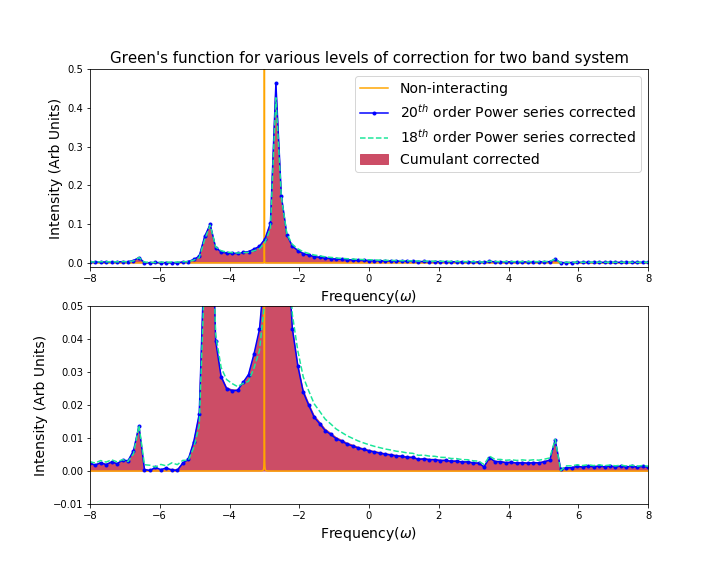
\includegraphics[width = 0.7\textwidth]{Single_boson_two_band_ret_cml.png}
    \caption{Numerically computed $20^{th}$ order retarded cumulant solution converges exactly to the predicted expression for retarded cumulant. Any more power series update just results in the same function. }
    \label{retarded cumulant}
\end{figure}

\section{Details of Exact Diagonalization}
In this section, we will briefly outline the construction of the two orbital Holstein Hamiltonian and the process of exact diagonalization. For a system with a single electron, N number of (+) bosons and N number of (-) bosons, there are three different components in the wave function - one for the electron and two for the two different bosons. For single electron, the electron wave function has three distinct entries each of which can either be 0 or 1. This is because of Pauli exclusion principle.
\begin{equation}
\begin{aligned}
    \ket{\psi_e} &=\ket{n_v, n_+, n_-} \qquad \text{where,}\\
    n_v &= \text{vacuum designator}\\
    n_+ &= \text{+ orbital designator}\\
    n_- &= \text{- orbital designator}\\
\end{aligned}
\end{equation}

Here, if there are no electrons in the system $n_v =1$ denoting electron vacuum. Presence of any electron in the system implies that $n_v =0$. If the electron is in $+$ orbital, $n_+ =1$ and otherwise $n_+=0$. Similarly, if the electron is in $-$ orbital, $n_- =1$ and otherwise $n_-=0$. For bosons, there is no restriction on the number of bosons that can coexist at a time. But for the sake of exact diagonalization, we need to enforce a cutoff that the maximum possible boson number is N in order to cutoff the Hamiltonian- the idea being that as $N\rightarrow\infty$, this finite Hamiltonian's eigenvalues approaches the exact eigenvalues. Any given $m^{th}$ wave function denoting that there are "m" bosons in the system for the ($\pm$) boson is as follows;
\begin{equation}
\begin{aligned}
    \ket{\Phi_\pm} &= \ket{n_0,n_1, n_2, n_3,..,n_m,..,n_{N-1},n_N} \quad\text{where,}\\
    n_m &= 1\\
    n_{k\neq m} &=0
\end{aligned}
\end{equation}
Here $n_0=1$ indicates boson vacuum. Since our boson wave function is based on the boson number rather than states, at any given time, only one of the $n_i$ can be non-zero. For instance, if there are two (+) bosons, only $n_2=1$ and all other $n_{i\neq 2} = 0$. For the entire single electron two plasmon bath system, any total wave function is then;
\begin{equation}
    \ket{\Psi(a,b,c)} = \ket{\psi_e^a} \bigotimes \ket{\Phi_+^b} \bigotimes \ket{\Phi_-^c}
\end{equation}
Here, $0\leq b,c \leq N$ by construction. In this system, there are $3(N+1)^2$ basis vectors. Because the Hamiltonian matrix scales as $(N+1)^2$,computation becomes exceedingly expensive with increasing boson number. 
\begin{figure}
    \centering
    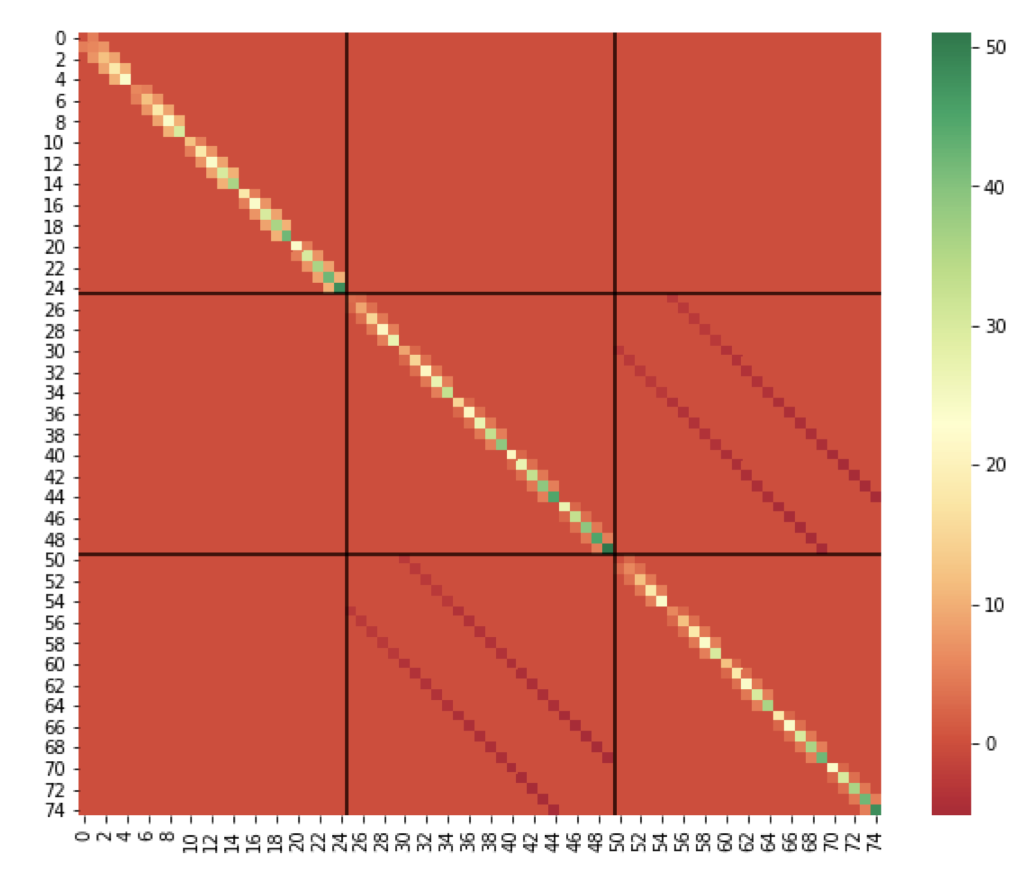
\includegraphics[width = 0.7\textwidth]{Hamiltonian.001.png}
    \caption{Hamiltonian with maximum of 4 plasmons
    (bosons) in each plasmon species ($\pm$) is already a $75\times75$ matrix}
    \label{4 boson H}
\end{figure}

Once, we construct this Hamiltonian, we can then find the eigenvalues and eigenvectors for it. The eigenvalue-eigenvector pair is represented as $\{\varepsilon_i, \ket{i}\}_i$ and there are $3(N+1)^2$ of them. The choice of boson number is dependent on the energy scale that we are looking at. With increasing $N$, we get the ability to resolve events closer in energy at the expense of computation time. At large plasma frequency, events happen far apart from each other and hence we only need a few bosons to resolve the system properly. At small plasma frequency however, since plasmonic shake offs are very close to each other, we need a large number of bosons to properly resolve such events.
\begin{figure}[H]
    \centering
    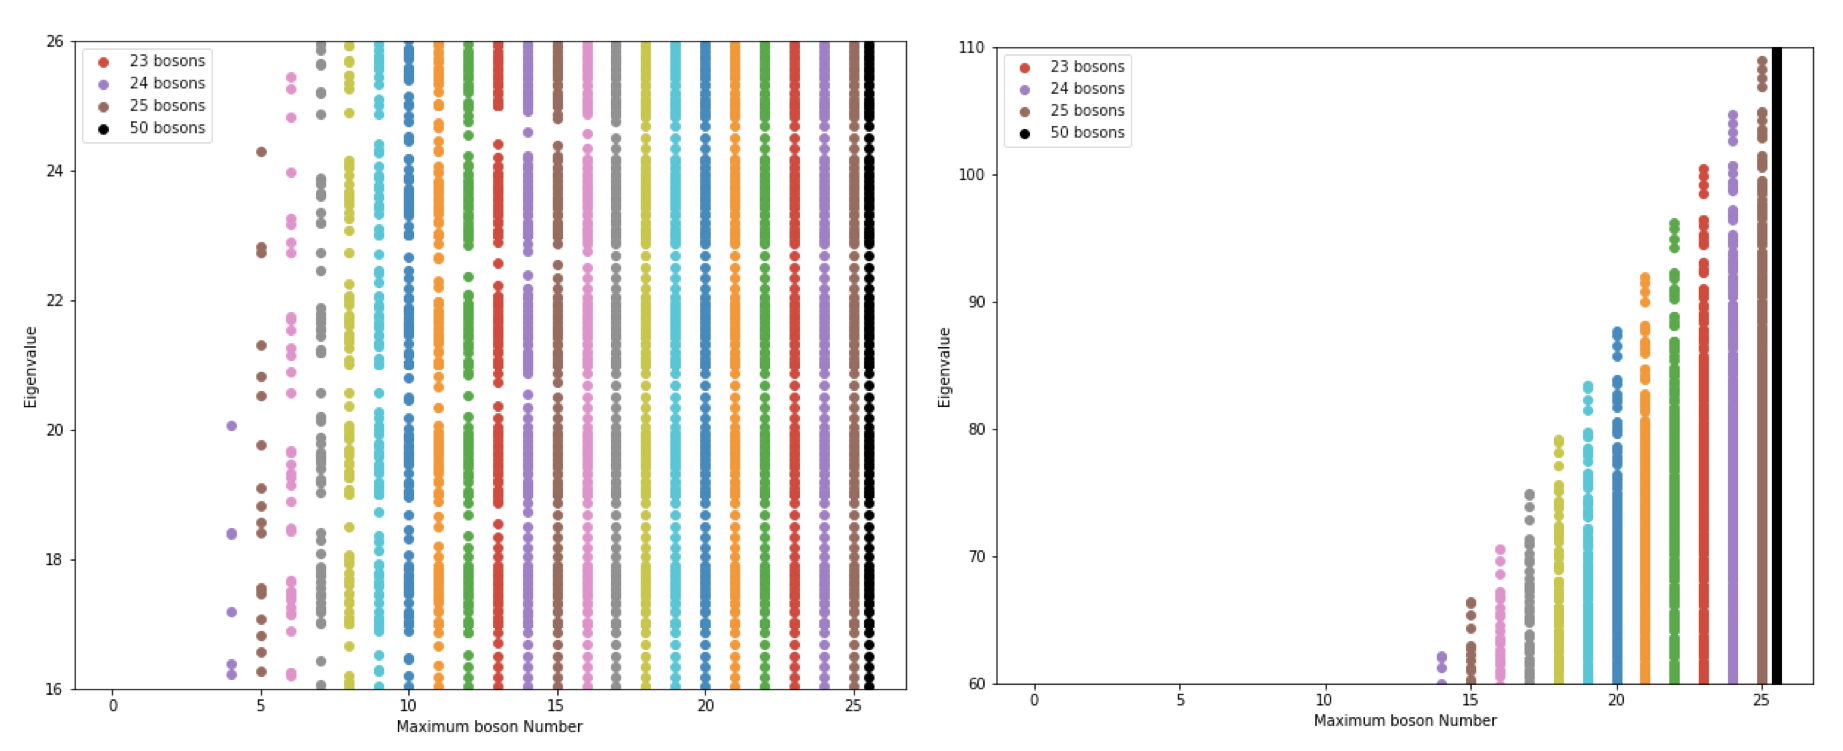
\includegraphics[width = 0.9\textwidth]{Eigenvalue.001.png}
    \caption{With increasing boson number, the eigenvalue differences between different sized system becomes smaller and smaller. The noticeable difference in above figures between different sized systems are only at large eigenvalues that lie in the eigenvalue continuum (right).}
    \label{Eigenvalue_spectra}
\end{figure}

Finally, we are in a position to compute the single particle Green's function. Here $\ket{0}$ implies total vacuum (Fermion as well as boson vacuums' outer product).

\begin{equation}
\begin{aligned}
    G(m,n;t) &= -i \theta(t)\left\langle 0|\{c_m(t) ,{c_n^{\dagger}}\}|0\right\rangle\\
    &= -i \theta(t)\left\langle 0|\{e^{iHt}c_m e^{-iHt} ,{c_n^{\dagger}}\}|0\right\rangle\\
    &= -i \theta(t)\sum_i\sum_j\left\langle 0|\{e^{iHt}\ket{i}\bra{i}c_m \ket{j}\bra{j}e^{-iHt} ,{c_n^{\dagger}}\}|0\right\rangle\\ 
\end{aligned}
\label{Greens definition}
\end{equation}
The only piece that survived in this Green's function after we open the anti-commutator is given by,
\begin{equation}
\begin{aligned}
    G(m,n;t)
    &= -i \theta(t)\sum_i\sum_j\left\langle 0|e^{iHt}\ket{i}\bra{i}c_m \ket{j}\bra{j}e^{-iHt} ,{c_n^{\dagger}}|0\right\rangle\\ 
    &= -i \theta(t)\sum_i\sum_j\left\langle 0|e^{i\varepsilon_it}\ket{i}\bra{i}c_m \ket{j}\bra{j}e^{-i\varepsilon_j t} ,{c_n^{\dagger}}|0\right\rangle\\ 
\end{aligned}
\label{Greens definition RT}
\end{equation}
This is the Green's function from exact diagonalization that we plot in our work.

\bibliography{Power_Series_5}

\end{document}
